\section{Introduction}
\label{sec:intro}

Consider a data warehouse scenario: a database describes how a set of \emph{measures} varies along several \emph{dimensions}. To work with this database, analysts need a lot of prior knowledge: which dimensions and measures they are interested in, where interesting patterns are hidden in the cube, which dependencies among dimensions and measures exist, and many more. Even a very experienced analysts might not have this prior knowledge as data distributions change over time and the interesting patterns to discover in the data cube are simple unknown to the human user. Focusing on the traditional manual exploration will detect unexpected patterns only by chance and not with a systematic search. In contrast to this, we aim at a semi-automated exploration that assist the humans in understanding how measures are distributed, where unexpected measures appear, and where interesting dependencies between dimensions and measures arise.

We believe that automatic query generation is essential to make data analysts more
productive. Informations which are trivial for domain experts are not
necessarily so for data specialists. Besides, experts themselves may need
guidance. Consider for instance Figure \ref{intro}. The table shows a small
extract from a dataset of astronomical observations\footnote{This dataset come
from the LOFAR research programme, 21 May 2012, the Netherlands}. This set
describes the \emph{luminosity} of more than 100,000 sources, taken at
different times, frequency ranges and with different precisions. In total,
there are more than fifty dimensions. Even for an astronomer, this dataset
cannot be understood by intuition alone. We need intelligent tools
to provide guidance.  The bottom picture illustrates what
we expect from our query generation system: a simpler low dimension view of dependent dimensions and measures, which reveals
particularly bright or large sources. Thanks to this view, anyone can 
quickly perceive interesting regions in the database.

\begin{figure}[t!]
\centering
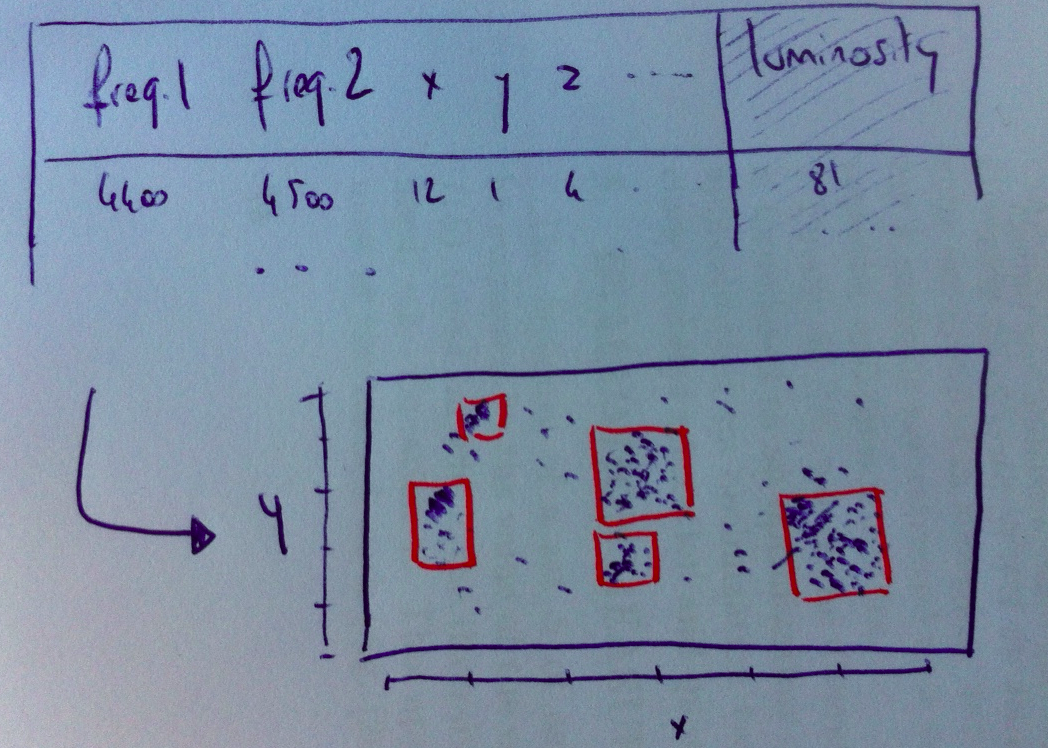
\includegraphics[width=0.8\columnwidth]{images/intro}
\caption{Revealing interesting regions}
\label{intro}
\end{figure}

Automatic query generation for a semi-automated exploration of data cubes is fundamentally challenging for two reasons. The first
reason is obvious: how do we define ``interestingness''?  The diversity of
opinions in the literature is rather depressing. What is interesting for a
user can be extremely boring for another. The second problem is practical.
Even if we had a universal measure of interest, how could we explore the search
space fast enough to find the interesting queries?

Many authors have proposed semi-automated (or discovery-driven) data cubes in the past.  A seminal work was
presented by Sarawagi et al. \cite{sarawagi1998discovery}. According to their
paper, the most interesting queries are the most ``surprising'' ones.
Therefore, they propose to build a (log-linear) model over the data, and
identify the largest deviations. More recently, Dash et
al.\cite{dash2008dynamic} proposed a facet selection method, also based on
surprise. These papers have a trait common: they set a model of
interestingness, and the exploit the particularities of their model to speed up
the computations. Nevertheless, are these interestingness models \emph{really}
interesting for the users?

In this paper, we propose to \emph{abstract interestingness away}. We introduce
\textit{Claude}, our generic query generation system. Claude's model is much simpler
that its predecessors. A user gives one, or several \emph{measures of
interest}. Claude finds the regions and dimensions with the largest deviations. Claude's
strength comes from its generality. In our example, the measure can describe the luminosity of a
star, its deviation from a log-linear model (cf. Sarawagi et al.) or anything
else. Thus, \emph{we let the user decide what is interesting for exploration, and we assist on
the systematic search}. Because of the generic design of our approach, performance is a major
challenge. We introduce two algorithms. The first one is exact and based on a systematic
level-wise search paradigm. The second one is a much faster and based on a relaxation of our model and a heuristic search.
